\chapter{Evolutionary dynamics on graphs}
\label{chp:nature} 
\cite{lieberman2005evolutionary}
Tanker fra paper:

To be able to point out insurable topologies, an extensive study of different graphs and how they behave has to be conducted. Regarding security, knowledge of how viruses spread and how to use graph structures to prevent malicious hackers from entering your network is important. Evolutionary dynamics, and the research of how mutant genes spread though out a population fits in to the model of security. 

From population studies \cite{lieberman2005evolutionary}, advantageous mutant e.g a virus inserted in circulation graph, will have a fixation probability equal to
\begin{equation}  p_{1}=\frac{(1-1/r)}{(1-1/r^{N})} \label{eq:fixation} \end{equation}

Where the fixation probability determines the rate of evolution, which relies both on the size of the network and the evolution speed. A probability of 1 means that every node in the network eventually will be affected by the mutant.   


Isotherm graphs are a sub-graph of circulation. 


If $W$ is symmetric, or isotherm then the fixation probability is always \ref{eq:fixation}
isotherm means doubly stochastic, all rows and cols sum to 1. 
If a graph is one rooted, it has a fixation prob of $1/N$ regardless of $r$. If a graph has more then one root, its fixation probability is zero. 
Is it possible to find graphs with fixation probability that exceeds \ref{eq:fixation}? Is it possible to suppress drift and amplify selection?
In a star-topology \ref{fig:star} the fixation probability is\begin{equation}p_{2}=\frac{(1-1/r^{2})}{(1-1/r^{2N})} \label{eq:fixation2} \end{equation}.
or more generally: \begin{equation}
p_{k}=\frac{(1-1/r^{k})}{(1-1/r^{kN})} \label{eq:fixationk}
\end{equation}

And the selective difference is as we see amplified from $r$ to $r^{2}$. i.e. a star act as an evolutionary amplifier,
 favoring advantageous mutants and inhibiting disadvantageous mutants, tilts towards selection and against drift.
 in certain graphs, star, funnel, metafunnel, if N is large enough, fixation probability for advantageous mutant converges to 1. Fixprob for disadvantageous converges to 0.
The same theory can be used to demonstrate how the aggregated security of a network is higher if the central node of a star structure is secured. 
If we assume that implemented security is 100$%$ efficient, no threats will propagate beyond that node i.e total security for the network is increased. 
 
This could maybe be used to show that if we have a star, funnel, metafunnel or something, and we secure the nodes it could force the virus to die out?
Scale-free networks have most of their connectivity clustered in a few vertices, i.e. they are potent selection amplifiers.
More generalized, $W$ does not need to be stochastic, $w_{ij}>=0$. 
If the sum of all edges leaving a vertex is equal for all vertexes, then the graph will never suppress selection.
If the sum of all edges entering a vertex is equal for all vertexes, the graph never suppress drift.
If both then the graph is called a circulation.
 
The game:
The way this game works, is that we look at nodes that are mutated (A), and those who are not (B).  
\begin{figure}
\centering 
\begin{tabular}{ l | c | r }
  
   & A & B \\  \hline  
  A & a & b \\ \hline  
  B & c & d \\
  
\end{tabular}
\caption{\label{fig:gamesetup} Setup propagation game \cite{lieberman2005evolutionary}}
\end{figure}

When we apply the game to a directed graph, there are four different outcomes, a,b,c and d, which represents the interaction between the nodes, as is depicted in the figures below\ref{fig:game}. 

In the first figure (Positive symmetric) the fixation probability is related to r=b/c. If b is greater than c, the properties of mutant b will propagate in to all the other nodes, and the whole graph will eventually consists of only mutated nodes. The opposite will happen in the case where c is greater than b, leading to extinction of the mutation. The later scenario models the situation where proper protection against a mutant i.e. a security threat is installed. If the level of security, c is higher that the strength of the security threat it will be blocked from propagating further into the network. 

\begin{figure}
\centering
\begin{tabular}{@{}c@{}}
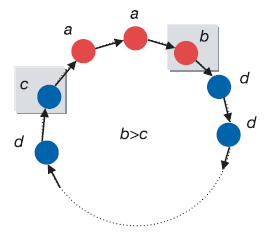
\includegraphics[width=1.0\textwidth]{natureGameSingle.png}
\end{tabular}
\caption{\label{fig:game} Mutant propagation game}
\end{figure}


\begin{figure}
\centering
\begin{tabular}{@{}c@{}}

\includegraphics[width=0.5\textwidth]{NetworkTopology-Star.png}
\end{tabular}
\caption{\label{fig:star} A star-topology}
\end{figure}



